%\documentclass[a4paper,12pt,oneside,draft]{article}
\documentclass[a4paper,12pt,oneside]{article}

% In the original writelatex tamplate
\usepackage[english]{babel}
\usepackage[utf8]{inputenc}
\usepackage{amsmath}
\usepackage{graphicx}
\usepackage[colorinlistoftodos]{todonotes}

% By LoCigno
\usepackage{times}
\usepackage{graphicx}
\usepackage{subfigure}
\usepackage{color}
\usepackage{url}
\usepackage{cleveref}

% By Davide
\usepackage{comment}
\usepackage{booktabs}
\usepackage{color}

%Variables macros
\newcommand{\DefineVar}[2]{%
  \expandafter\newcommand\csname var-#1\endcsname{#2}%
} 
\newcommand{\var}[1]{\csname var-#1\endcsname}

\usepackage{courier}
\newcommand{\mono}[1]{\texttt{#1}}
%\newcommand{\mono}[1]{\texttt{\textbf{#1}}}

\title{Identification procedure for Lego Mindstorm motor}

\author{Diego Verona, Aliaksandr Siarohin, Mattia Digilio}

\date{\today}

\begin{document}
%\maketitle
\makeatletter  % populates \@title, \@author, \@date
\begin{titlepage}
      \centering
      ~~~~~~~~~~~~~\\[-30mm]
      
\includegraphics[keepaspectratio=true, width=7cm]{bg_eng_1r.jpg} \\[10mm]

     {
     \large \bfseries Master Degree in Computer Science\\[3mm] 
     Applied Robotics\\[3mm]
     AA 2015-2016
     }\\[10mm]

     %--------------------------------
     % Set the title, author, and date
     % 

     \vspace{0.5cm}
     {
     \Large \bfseries \textcolor{blue}{\@title} \par
     }
     \vspace{0.5cm}
%      {
%      \large {Group N. 1} \par
%      }
     \vspace{0.2cm}

     {\large {\@author}}
     \\ \vspace{.2cm}
     \@date

     \vspace{0.6cm}

    %-----------------------------------

\begin{abstract}

\textit{
  Report for the first assigment on Applied robotics. Identification parameters of the motor. In this report we disscuss our method of obtaining the data from Lego Mindstorm motor as well as estimation of parameters from the motor  data.
}


\end{abstract}

\end{titlepage}

\section{Collecting motor data}
We use 2 methods for collecting the motor data:
\begin{enumerate}
\item Using the bluetooth connection
\item Using usb connection
\end{enumerate}

\subsection{Bluetooth data collection}
We start from the brofist source, and we change message interface to include timestamp. The idea is follows:
\begin{enumerate}
\item Send message that tells motor to set up specific power.
\item Send message that requests tacho count from the motor.
\item Receive tacho count with timestamp.
\item Save (timestamp, tacho count) to file.
\item Go to step 2.
\end{enumerate}
You can find code in \url{https://github.com/AliaksandrSiarohin/AppliedRobotics/brofist}. But using this methodology we obtain very hight latency $\approx 50ms$. So we decided to use USB conection instead.

\subsection{USB data collection}
We use library pyusb to establich usb conection with brick. The idea is folows:
\begin{enumerate}
\item Establish connection with brick using pyusb.
\item Setup the motor power on the brick.
\item Send (timestamp,  tacho count) from brick.
\item Receive (timestamp,  tacho count)  at PC.
\item Save (timestamp,  tacho count) to file.
\item Go to step 3.
\end{enumerate}
You can find code in \url{https://github.com/AliaksandrSiarohin/AppliedRobotics/usb_collector}. Using this methodology we obtain much better perfomance $\approx 2ms$ latency. Using USB we collect 10 data files with different raw powers.

\section {Estimating the parameters from the data}
To estimate the parameters we filter the data using butterworth filter and then we estimate the parameters using 2 methods:
\begin{itemize}
\item Regular method proposed on the lecture
\item Regression method
\end{itemize}

\subsection {Filtering}
We use butterwoth filter of order 1 and and cut-off frequency 0.02. For example \cref{fig:filterd}.
\begin{figure}[t]%
	\centering
	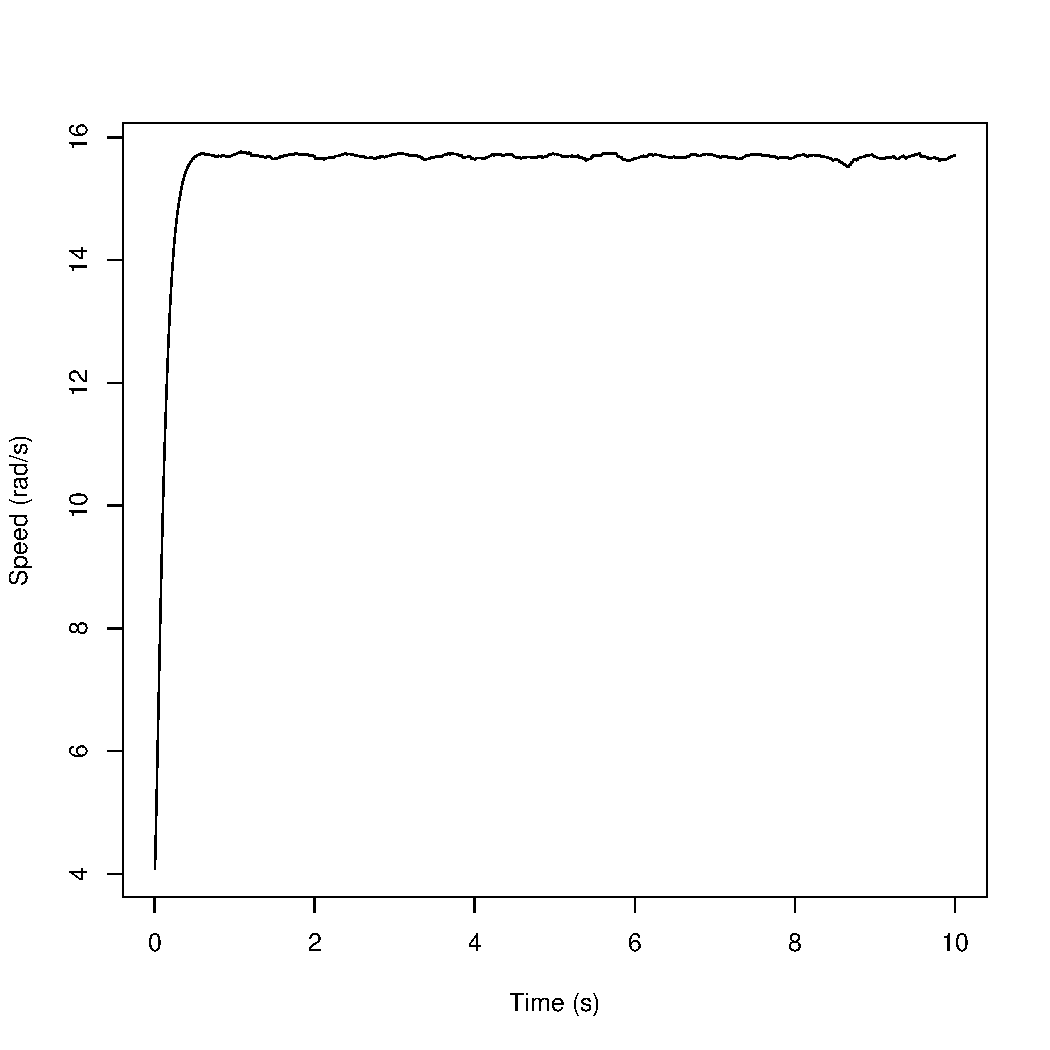
\includegraphics[width=\columnwidth]{~/apr/AppliedRobotics/motor_data/plots/v90_20000.pdf}
	\caption{Deviation of x from it`s mean.}%
	\label{fig:filtered}%
\end{figure}


\end{document}